
\begin{figure}[H]
  \label{fig:benaderingen}
  % Set the overall layout of the tree
  \tikzstyle{level 1}=[level distance=2.5cm, sibling distance=3.5cm]
  \tikzstyle{level 2}=[level distance=2cm, sibling distance=2cm]
  \tikzstyle{level 3}=[level distance=3cm, sibling distance=3cm]
  \tikzstyle{level 4}=[level distance=2cm, sibling distance=2cm]
  \tikzstyle{level 5}=[level distance=2cm, sibling distance=2cm]
  \tikzstyle{level 6}=[level distance=2cm, sibling distance=2cm]

  % Define styles for bags and leafs
  \tikzstyle{bag} = [text width=3em,text centered]
  \tikzstyle{end} = [minimum width=3pt,fill, inner sep=0pt]

  % The sloped option gives rotated edge labels. Personally
  % I find sloped labels a bit difficult to read. Remove the sloped options
  % to get horizontal labels. 
  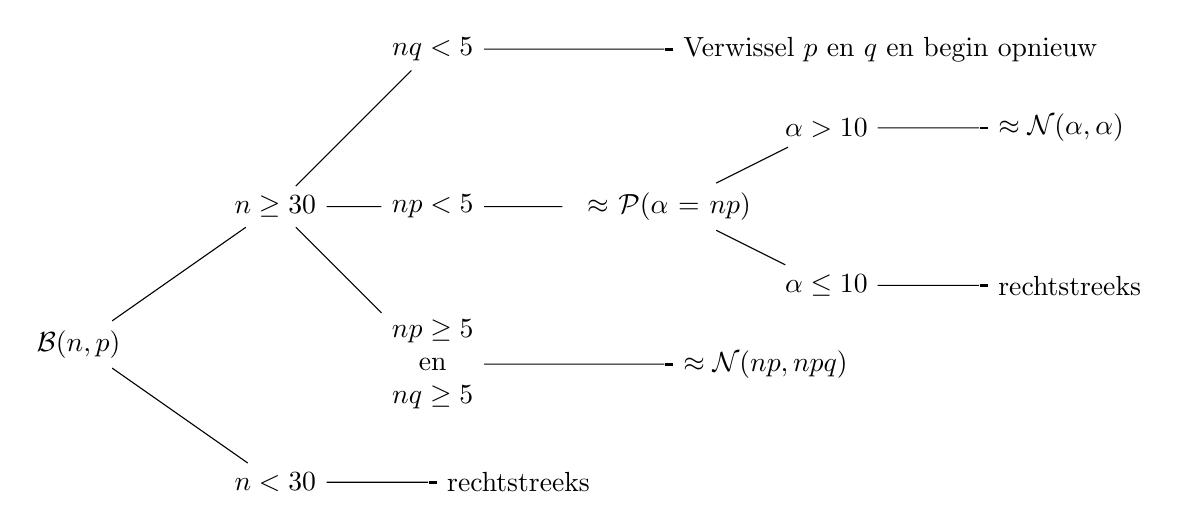
\begin{tikzpicture}[grow=right, sloped]
    \node[bag] {$\mathcal{B}(n,p)$}
    child {
      node[bag] {$n < 30$}        
      child {
        node[end, label=right:{rechtstreeks}] {}
      }
    }
    child {
      node[bag] {$n \ge 30$}        
      child {
        node[bag] {$np \ge 5$ en $nq \ge 5$}
        child {
          node[end, label=right:{$\approx \mathcal{N}(np,npq)$}] {}
        }
      }
      child {
        node[bag] {$np < 5$}
        child {
          node[bag, text width=7em] {$\approx \mathcal{P}(\alpha=np)$}
          child {
            node[bag] {$\alpha \le 10$}
            child {
              node[end,label=right:{rechtstreeks}] {}
            }
          }
          child {
            node[bag] {$\alpha > 10$}
            child {
              node[end, label=right:{$\approx \mathcal{N}(\alpha,\alpha)$}] {}
            }
          }
        }
      }
      child {
        node[bag] {$nq < 5$}
        child {
          node[end, label=right:{Verwissel $p$ en $q$ en begin opnieuw}] {}
        }
      }
    };
  \end{tikzpicture}
\end{figure}